\documentclass[addpoints]{exam}

\usepackage{epic,array,ecltree,url, calrsfs}
\usepackage[nointegrals]{wasysym}
\usepackage{mlextra}


%These tell TeX which packages to use.
\usepackage{epsfig}
\usepackage{amsmath}
\usepackage{amsfonts}
\usepackage{amssymb}
\usepackage{amsxtra}
\usepackage{amsthm}
\usepackage{mathrsfs}
\usepackage[dvipsnames]{xcolor}
\usepackage{array}
\usepackage{graphicx}
\graphicspath{ {../art/} }
\usepackage{bm}
\usepackage{tikz}
\usepackage{multicol}

\renewcommand\qedsymbol{$\blacksquare$}

%Here I define some theorem styles and shortcut commands for symbols I use often
\theoremstyle{definition}
\newtheorem{defn}{Definition}
\newtheorem{thm}{Theorem}
\newtheorem{cor}{Corollary}
\newtheorem*{rmk}{Remark}
\newtheorem{lem}{Lemma}
\newtheorem*{joke}{Joke}
\newtheorem{ex}{Example}
\newtheorem*{soln}{Solution}
\newtheorem{prop}{Proposition}

\newcommand{\lra}{\longrightarrow}
\newcommand{\ra}{\rightarrow}
\newcommand{\surj}{\twoheadrightarrow}
\newcommand{\graph}{\mathrm{graph}}
\newcommand{\bb}[1]{\mathbb{#1}}
\newcommand{\Ell}{\mathscr{L}}
\newcommand{\Z}{\bb{Z}}
\newcommand{\Q}{\bb{Q}}
\newcommand{\R}{\bb{R}}
\newcommand{\C}{\bb{C}}
\newcommand{\N}{\bb{N}}
\newcommand{\M}{\mathbf{M}}
\newcommand{\m}{\mathbf{m}}
\newcommand{\MM}{\mathscr{M}}
\newcommand{\HH}{\mathscr{H}}
\newcommand{\Om}{\Omega}
\newcommand{\Ho}{\in\HH(\Om)}
\newcommand{\bd}{\partial}
\newcommand{\del}{\partial}
\newcommand{\bardel}{\overline\partial}
\newcommand{\textdf}[1]{\textbf{\textsf{#1}}\index{#1}}
\newcommand{\img}{\mathrm{img}}
\newcommand{\ip}[2]{\left\langle{#1},{#2}\right\rangle}
\newcommand{\inter}[1]{\mathrm{int}{#1}}
\newcommand{\exter}[1]{\mathrm{ext}{#1}}
\newcommand{\cl}[1]{\mathrm{cl}{#1}}
\newcommand{\ds}{\displaystyle}
\newcommand{\vol}{\mathrm{vol}}
\newcommand{\cnt}{\mathrm{ct}}
\newcommand{\osc}{\mathrm{osc}}
\newcommand{\LL}{\mathbf{L}}
\newcommand{\UU}{\mathbf{U}}
\newcommand{\support}{\mathrm{support}}
\newcommand{\AND}{\;\wedge\;}
\newcommand{\OR}{\;\vee\;}
\newcommand{\Oset}{\varnothing}
\newcommand{\st}{\ni}
\newcommand{\wh}{\widehat}

\newcommand{\id}[1]{\mbox{\it #1\/}}
\newcommand{\rid}[1]{\mbox{\rm #1}}
\newcommand{\sid}[1]{\mbox{\sf #1}}
\newcommand{\bid}[1]{\mbox{\bf #1}}
\newcommand{\tinysz}[1]{\mbox{\tiny $#1$}}

%Pagination stuff.
\setlength{\topmargin}{-.3 in}
\setlength{\oddsidemargin}{0in}
\setlength{\evensidemargin}{0in}
\setlength{\textheight}{9.in}
\setlength{\textwidth}{6.5in}



%\pagestyle{empty} 
%\footer{}{\thepage}{}

\newcommand{\twonode}{%
  \begingroup\normalfont
  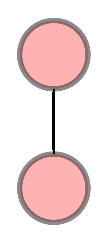
\includegraphics[height=\fontcharht\font`\b]{2nodetree.eps}%
  \endgroup
}

\newcommand{\tf}[1][{}]{%
\fillin[#1][0.25in]%
}
\noprintanswers
\unframedsolutions
\SolutionEmphasis{\itshape\small}
\SolutionEmphasis{\color{NavyBlue}}
\checkboxchar{$\Box$}
\checkedchar{$\blacksquare$}
\begin{document}


\noindent
\begin{tabular*}{\textwidth}{l @{\extracolsep{\fill}} r @{\extracolsep{6pt}} l}
{\large CS3920: Foundations of Computer Science} &  \makebox[3in]{\large Name:\enspace\hrulefill}\\
{\large June 11, 2018} & \\
{\large Quiz 5} & 
\end{tabular*}\\

\fbox{\fbox{\parbox{6in}{\textbf{Instructions}: Please answer the questions 
  below to the best of your ability. Be sure to show your work where appropriate. 
   This quiz is closed book, closed notes, closed computer. There are \numpoints\ 
   points in total. }}}\\
\begin{questions}
\question[2] Define propositions $p$ and $q$ as follows:\\
 $p$: ``Process p is in the critical section.''\\
 $q$: ``Process q is in the critical section.''\\ 

Write a statement in linear temporal logic that uses $p$ and $q$ to express the property of mutual
exclusion.
\vspace{20mm}

\question[4] Consider the following LTL formula: 
\[(\Box p \imp \Box q) \imp \Box(p \imp q)\]

For each of the interpretations below, mark $S$ if the interpretation satisfies
the formula, and $F$ if it falsifies the formula.(Assume the values of the last two 
states continue to repeat after $s_4$, so $s_5 = s_3$, $s_6 = s_4$, etc.)

\begin{choices}

\choice 
\unitlength=.9pt
\begin{picture}(340,30)
\put(  0,-5){\state{}{$s_{0}$}}
\put( 20, 5){\vector(1,0){40}}
\put( 60,-5){\state{}{$s_{1}$}}
\put( 80, 5){\vector(1,0){40}}
\put(120,-5){\state{}{$s_{2}$}}
\put(140, 5){\vector(1,0){40}}
\put(180,-5){\state{}{$s_{3}$}}
\put(200, 5){\vector(1,0){40}}
\put(240,-5){\state{}{$s_{4}$}}
\put(260, 5){\vector(1,0){40}}
\put(300, 0){\makebox(20,10){\ldots}}
\end{picture}
\tf (S/F)

\choice
\unitlength=.9pt
\begin{picture}(340,30)
\put(  0,-5){\state{}{$s_{0}$}}
\put( 20, 5){\vector(1,0){40}}
\put( 60,-5){\state{}{$s_{1}$}}
\put( 80, 5){\vector(1,0){40}}
\put(120,-5){\state{$p$}{$s_{2}$}}
\put(140, 5){\vector(1,0){40}}
\put(180,-5){\state{}{$s_{3}$}}
\put(200, 5){\vector(1,0){40}}
\put(240,-5){\state{}{$s_{4}$}}
\put(260, 5){\vector(1,0){40}}
\put(300, 0){\makebox(20,10){\ldots}}
\end{picture}
\tf (S/F)


\choice
\unitlength=.9pt
\begin{picture}(340,30)
\put(  0,-5){\state{$p$}{$s_{0}$}}
\put( 20, 5){\vector(1,0){40}}
\put( 60,-5){\state{$p$}{$s_{1}$}}
\put( 80, 5){\vector(1,0){40}}
\put(120,-5){\state{$p$}{$s_{2}$}}
\put(140, 5){\vector(1,0){40}}
\put(180,-5){\state{$p$}{$s_{3}$}}
\put(200, 5){\vector(1,0){40}}
\put(240,-5){\state{$p$}{$s_{4}$}}
\put(260, 5){\vector(1,0){40}}
\put(300, 0){\makebox(20,10){\ldots}}
\end{picture}
\tf (S/F)

\choice
\unitlength=.9pt
\begin{picture}(340,30)
\put(  0,-5){\state{$p$}{$s_{0}$}}
\put( 20, 5){\vector(1,0){40}}
\put( 60,-5){\state{$p$}{$s_{1}$}}
\put( 80, 5){\vector(1,0){40}}
\put(120,-5){\state{}{$s_{2}$}}
\put(140, 5){\vector(1,0){40}}
\put(180,-5){\state{$p$}{$s_{3}$}}
\put(200, 5){\vector(1,0){40}}
\put(240,-5){\state{$p$}{$s_{4}$}}
\put(260, 5){\vector(1,0){40}}
\put(300, 0){\makebox(20,10){\ldots}}
\end{picture}
\tf (S/F)

\end{choices}

\vspace{5mm}
\question Consider the following transition function, $\delta$:
\begin{align*}
  \delta(s_0,a) = s_0,\;\;& \delta(s_0,b) = s_1 \\
  \delta(s_1,a) = s_0,\;\;& \delta(s_1,b) = s_1 
\end{align*}
\begin{parts}
\part[2] Draw the corresponding state transition diagram for $\delta$.
\vspace{20mm}
\part[2] Let $\hat{\delta}(s_0,w) = s_1$. Which of the following are possible
values of $w$ (circle all that apply)?

\begin{oneparchoices}
\choice $b$
\choice $bba$
\choice $aab$
\choice $ababababababab$
\end{oneparchoices}
\end{parts}

\end{questions}
\end{document}


